\documentclass{article}
\usepackage{amssymb}
\usepackage{amsmath}
\usepackage{hyperref}
\usepackage{enumerate}
\usepackage{graphicx}
\usepackage{float}


\begin{document}

\title{Data Visualization \\ Worksheet 1}
\author{\large Ilya Ilyankou \\ ilya.ilyankou@worc.ox.ac.uk}
\date{}

\maketitle

\section{Eigenfaces}

\begin{enumerate}
\item
For the purpose of the exercise, I chose photographs of 3 celebrities: Trump, Hitler, and the guy in the very first folder of the given dataset (it was him who I saw when I finally fixed the issue with eigenface normalization). After cropping and resizing all three images to 180x200, I converted each into a vector of 36000 dimensions whose values are grayscale pixel representations, and subtracted the mean face from the original dataset. I then computed the coefficients of how much each eigenface should contribute to the reconstructed image, and displayed the reconstructed image.

\begin{figure}[h!]
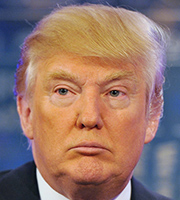
\includegraphics[height=2cm]{../trump}
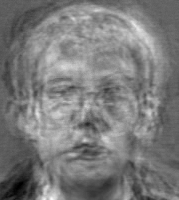
\includegraphics[height=2cm]{trump-recon}
\hspace{0.33cm}
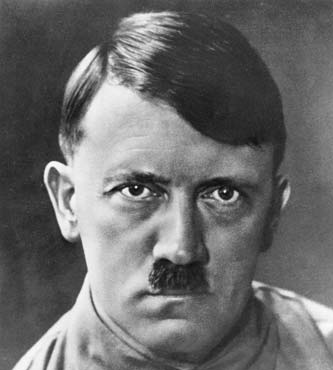
\includegraphics[height=2cm]{../hitler}
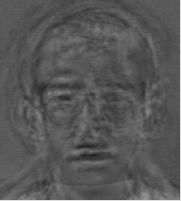
\includegraphics[height=2cm]{hitler-recon}
\hspace{0.33cm}
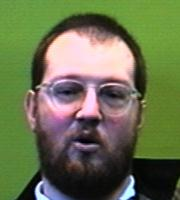
\includegraphics[height=2cm]{../guy0}
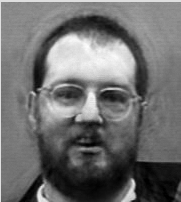
\includegraphics[height=2cm]{guy0-recon}
\caption{Representing Trump, Hitler, and Guy Zero using eigenfaces}
\end{figure}

\begin{itemize}
\item
Even when using all 113 eigenfaces, the images of Trump and Hitler are unrecognizable (can't say it's a bad thing). The image of Guy Zero is almost perfect, except that it almost completely repeats the image used to build the eigenfaces and does not capture his different facial expression.

\item
Obviously 113 vectors is not enough to build a universal face constructor. It is an extremely tiny dataset which is suitable for distinguishing faces which are in the dataset, but it is not nearly enough if we want to represent a brand-new face (hundreds of thousands, or even millions of eigenfaces are needed).

\item
Most of the background does not matter because it's the same on all headshots and thus deducted by the mean. So if we try to represent a face with busy background, we will fail, as no eigenfaces are capturing background features.

\end{itemize}

\item
Some of the advantages of eigenfaces are:
\begin{itemize}
\item
May be powerful for face recognition when we have headshots from specific positions (such as databases of mugshots).
\item
Can be used in file compression as using half or even a third of eigenfaces is often enough to be able to tell faces apart.
\item
Clear mathematics and easy implementation make it easy to use and justify how we got the result (unlike neural networks).
\end{itemize}

Some of the weaknesses of eigenfaces are:
\begin{itemize}
\item
Face recognition becomes nearly impossible when photos have different lighting, or people have different facial expressions, or turn or tilt their heads, etc.
\item
According to Wikipedia and my own observations, most significant eigenfaces do not represent some specific facial characteristics, but merely capture the lighting. Often the  three most significant eigenfaces are discarded.
\end{itemize}

\end{enumerate}


\section{Word Representations}

For this question, I trained Word2Vec on a dataset of subtitles to TED talks ($\approx$75MB). I decided to represent each word as a 29-dimensional vector instead of the standard 100D, because the PCA implementation of Python's \texttt{matplotlib} requires the number of samples (in my case, 30) to be greater than the number of dimensions.

I chose 30 words: 10 names of languages, 10 furniture items, and 10 cities.

\begin{enumerate}
\item

PCA produced quite decent mapping.

\begin{figure}[h!]
\begin{center}
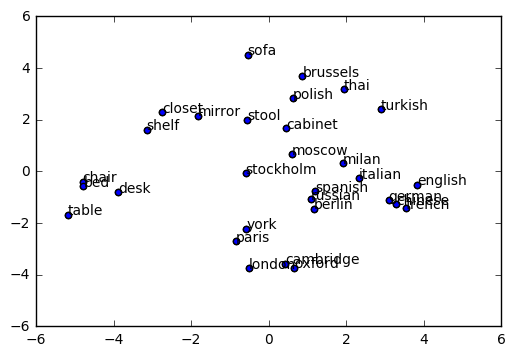
\includegraphics[height=7cm]{pca}
\end{center}
\caption{Mapping 29D words onto 2D using PCA}
\end{figure}

All furniture items are grouped together on the left side and can be circles with an ellipse. The cities and languages are mixed together, with cities being closer to furniture, and languages being on the right. English places (London, Cambridge, York, and Oxford) along with Paris create a cluster in the bottom center.

Considering that Word2Vec was trained on a relatively small dataset, and only 29 dimensions were used to capture the differences between the words, I did not expect to see three distinct clusters. I am satisfied with the obtained result.

Multidimensional Scaling also managed to place the words quite well. We can observe the same British cluster (Oxford, Cambridge, London, York), furniture creates a distrinct cluster and is separate from the rest of the words. All languages are in the lower right corner.

\begin{figure}[h!]
\begin{center}
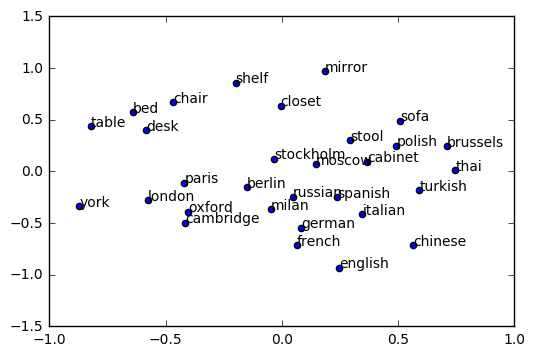
\includegraphics[height=7cm]{mds}
\end{center}
\caption{Mapping 29D words onto 2D using MDS}
\end{figure}

\item
Overall the two scatter plots look very similar. If one rotates Figure 2 $20^o-30^o$ anti-clockwise, the words will end up approximately in the same positions relative to the axes.

In MDS, however, all dots are scattered somewhat uniformly, whereas in PCA we can observe points clustered very close to each other: (Spanish, Russian, Berlin), (Oxford, Cambridge), (bed, chair), and (German, Chinese, French). This may signify that if one needs closer clustering of similar points, PCA may be a better choice.

MDS put York somewhat aside from other British places and Paris, whereas with PCA, York is extremely close to Paris.

\end{enumerate}

\end{document}